\section{Inicio de sesión de usuarios existentes y nuevos}

El inicio de sesión se comienza desde la pantalla de lanzamiento de la aplicación utilizando el botón destinado para tal fin. El proceso varía si el usuario es un usuario nuevo o si ya está registrado en el sistema y cuenta con un perfil completo. El flujo de actividades para el inicio de sesión global con ambos casos es el ilustrado en la \fref{dia:actividad_inicio_sesion}. Estos dos tipos de inicio de sesión se corresponden con los casos de uso \textbf{\nameref{sec:cu:registro}} y \textbf{\nameref{sec:cu:iniciar_sesion}}. 

El \textbf{inicio de sesión} estándar puede verse en detalle en el diagrama de secuencia de la \fref{dia:secuencia_inicio_sesion}. El proceso comienza con el usuario solicitando el inicio de sesión en la aplicación móvil, tras lo que se le solicitará una cuenta de Google para realizarlo. Una vez que se verifique la cuenta con la librería de autenticación de Google se enviará el \gls{token} de la sesión de Google a la \acrshort{api} por el \gls{endpoint} correspondiente. La \acrshort{api} usará dicho \gls{token} para obtener la ID única de Google del usuario, con la que consultará a la base de datos para recuperar el perfil de usuario almacenado. Con dicha información generará una nueva sesión que persistirá en la base de datos antes de enviarla como respuesta a la aplicación junto a los datos del usuario. Tras recibir la respuesta, la aplicación almacenará esa sesión y el usuario, y avanzará hasta la pantalla principal con la \textbf{sesión iniciada}. 

El \textbf{registro de nuevos usuarios} comienza igual que el inicio de sesión hasta la obtención de la ID de la cuenta de Google del usuario por parte de la \acrshort{api}. Tras esto, la consulta a la base de datos para recuperar el perfil no retornará ningún usuario, indicando que \textbf{dicho usuario no existe}. En ese momento, la \acrshort{api} creará un nuevo usuario con la ID de Google que persistirá antes de crear una sesión que enviar junto a dicho usuario incompleto. Al recibir un \emph{User} incompleto la aplicación dirigirá al usuario a la \textbf{SetUpActivity}. En dicha pantalla el usuario introducirá sus datos restantes, completando su perfil. Una vez confirme los datos enviados, la aplicación realizará la petición de parcheo a la \acrshort{api}, que persistirá dichos datos y devolverá el nuevo \emph{User} actualizado. El final de esta secuencia será como el del \textbf{inicio de sesión}, con el almacenamiento de dicho \emph{User} y el avance hasta la pantalla principal con la sesión iniciada en el nuevo perfil.

\begin{figure}
    \centering
    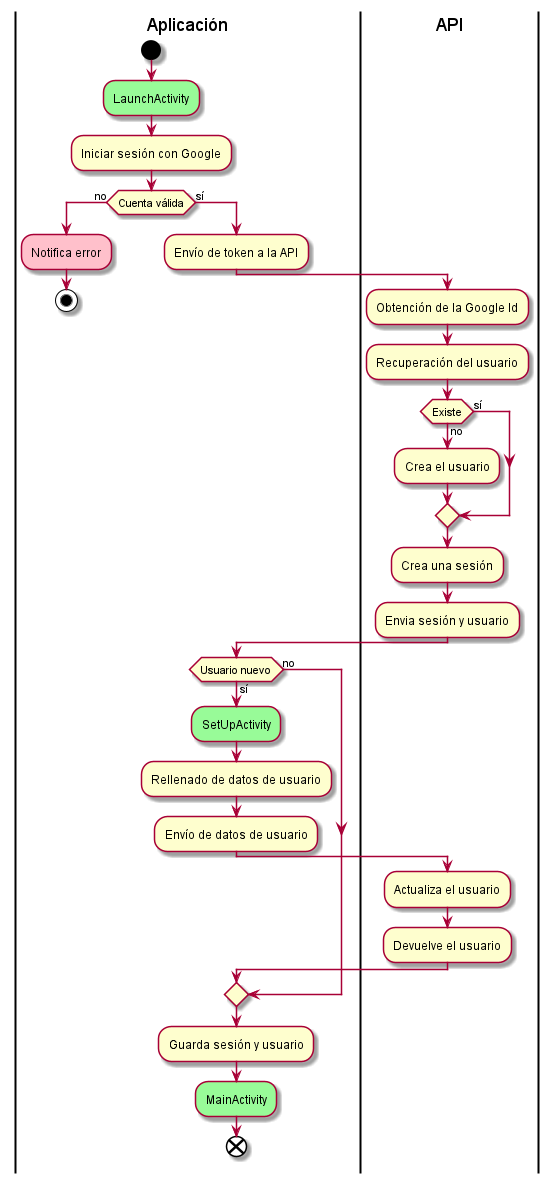
\includegraphics[width=0.65\textwidth]{images/Diseño/ActividadesInicioSesion.png}
    \caption{Diagrama de actividades del inicio de sesión}
    \label{dia:actividad_inicio_sesion}
\end{figure}

\begin{figure}
    \centering
    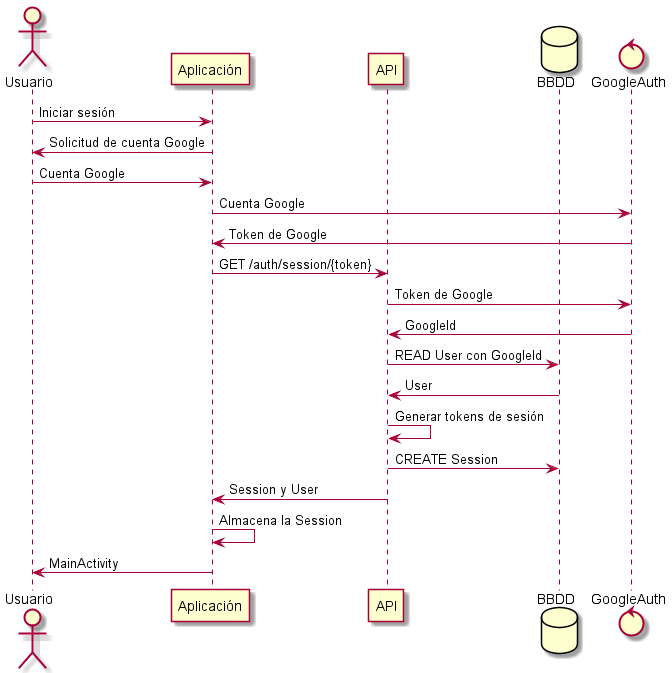
\includegraphics[width=0.5\textwidth]{images/Diseño/SecuenciaInicioSesion.png}
    \caption{Diagrama de secuencia del inicio de sesión}
    \label{dia:secuencia_inicio_sesion}
\end{figure}

\begin{figure}
    \centering
    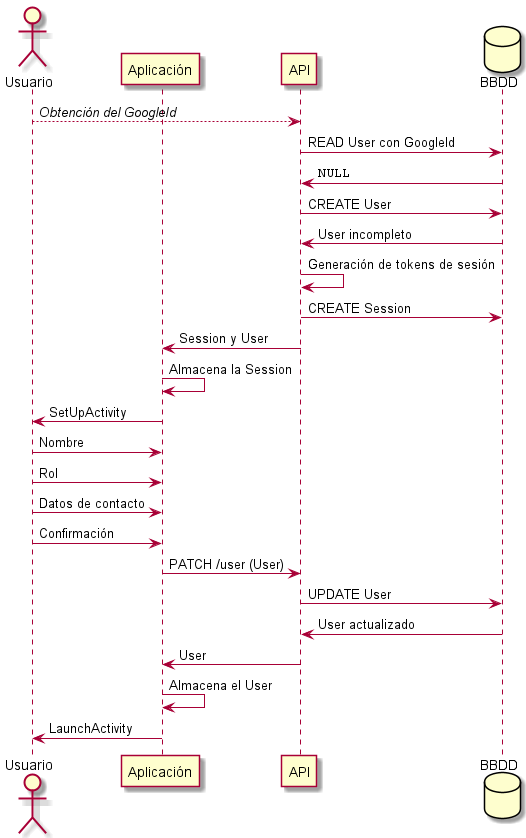
\includegraphics[width=0.5\textwidth]{images/Diseño/SecuenciaRegistro.png}
    \caption{Diagrama de secuencia de registro}
    \label{dia:secuencia_registro}
\end{figure}